\chapter{Methodology of Refactoring Process}

% Introduction Paragraph
The following part of this chapter moves on to describe in greater detail detection code smells within the software system. It provides a brief overview of the methods used for detection and mentions the prevalence of sonargraph as the main suite of software products utilized in the detection activities. Moreover, this section provides some clarifications necessary to comprehend certain methods to be chosen over others.

% Extension of the Refactoring process
- In the end it should be clear, why refactoring is tightly integrated in other development processes
- List this model; tell what is extra included
- This will also be a hypothesis (That we can extend our refactoring; see where it connects to optimize it) -> There are no indications about this in literature, as far as concerned (verify)

% Short decription of each part of process
-> Get an initial understanding


\section{Detecting Code Smells}


% Catalogue
Out of 24 code smells that are examined throughout Martin Fowler's book on refactoring, only 10 are chosen to be included in the detection work. Further, the 2 smells \emph{refused bequest} and \emph{data clumps} were discarded, as their focus on inheritance and data structures respectively, are not utilized in the code. In order to revisit the code smell catalog with their corresponding explanation, refer to (sec:...)
 

% Restrictions
There exists several reasons that have led to the decision of restricting the amount of smells for this section. First, it is not the scope of the thesis to find every code smell in the codebase. Finding and evaluating each smell that is known in literature would be a tedious task, as there are no automatic tools available for the python programming language, as will be discussed in a later part of this section. Hence, it suffices, if some smells that are prevalent have been detected. In addition, it is also advantageous to only focus on the most prominent smells. Very niche smells could distract from improving the quality of the entire code base, as well as provide less of possibilities to make generalizations.

% Metrics based
Many tools have been created to automatically or semi-automatically detect code smells (Menshawy, p.1). In the context of our paper, the code smells are detected semi-automatically using a metric-based approach. This approach measures source code elements and takes decisions based on threshold values (Menshawy, p.4) It is fulfills two requirements necessary for the following work. On the one hand, it to a certain degree contains automation, making it much more efficient in comparison to manual approaches. On the contrary, it can be used for the python programming language, which is essential in the software system at hand. Menshawy points out (p.3) that with metrics approach does not provide metrics for every code smells. Nevertheless, for the eight smells the thesis is focussing on, as will be seen afterwards, an appropriate metric was found.

% Automation based
Using a detection approach based on automated tools would have been more attractive, but unfortunately not possible.  It is the most used approach (Menshawy, p.2), its availability is however highly dependent on the programming language the software system is written in (Menshawy, p.3). By looking at Menshawy's research (p.3) on most cited tools, it can be observed that a significant difference exists between java programming language, which was supported  by 48\% of the tools, whereas the python programming language being only supported by 4\%.
In addition, by researching automated tools appropriate for python, it was evident that at this moment of time, the offering is insufficient for to accomplish a sound detection strategy. 

% Manual approach
In the beginning, the author has also considered following a manual approach. In contrast to automation, the manual detection relies on human perception of smells by applying predefined guidelines (Menshawy, p.3). It is characterized as highly time-consuming and prone to human error. Therefore, when comparing this approach to a metrics-based, it is a less desirable way for detecting smells and was subsequently discarded as a detection technique.

% Visualization
Another detection approach that has not yet been mentioned, is using visualization. Although it only is used to detect a subset of smells, visualization had been used in two occurrences throughout the thesis. First, it had been used to get a broad overview of the code base, which helped the author as an orientation. Second, it was used [... Add coupling + cohesion]

% Intro Sonargraph
The detection of code smells relied heavily on a code analyzer tool called sonargraph. It demonstrated to be extremely useful in the detection of code smells, by its ability to compute and list metrics of the software system. Countless metrics offered a diversity of selection, analyzing both on the basis of the entire project and individual modules. By reading through the provided explanations of the metric, an appropriate metric could be found for all the desired code smells relevant for the thesis.

% Explorer + Metrics
Compared to other software solutions, sonargraph was chosen for several reasons. Altough its entire product suite is not, its graphical application "Explorer" was free to use. For the thesis, it provided many ways to make observations about the code base, including numerical and visual methods. All the tools needed to compute metrics were restricted in this free application of the product family. In contrast, the detection of code duplication was not included within "Explorer". Nevertheless, although unsure about the amount, it was possible to renew a trial period multiple times. Hence, in order to recreate this method, one must be aware of this restriction. Another noteworthy benefit of using sonargraph during the detection, was its ability to observe the entire project,  and not just at individual files. This was essential for metrics taking account of dependencies between modules. In addition, it was beneficial not to rely on a multitude of software tools, by having just one software.



\begin{figure}[htp]
    \centering
    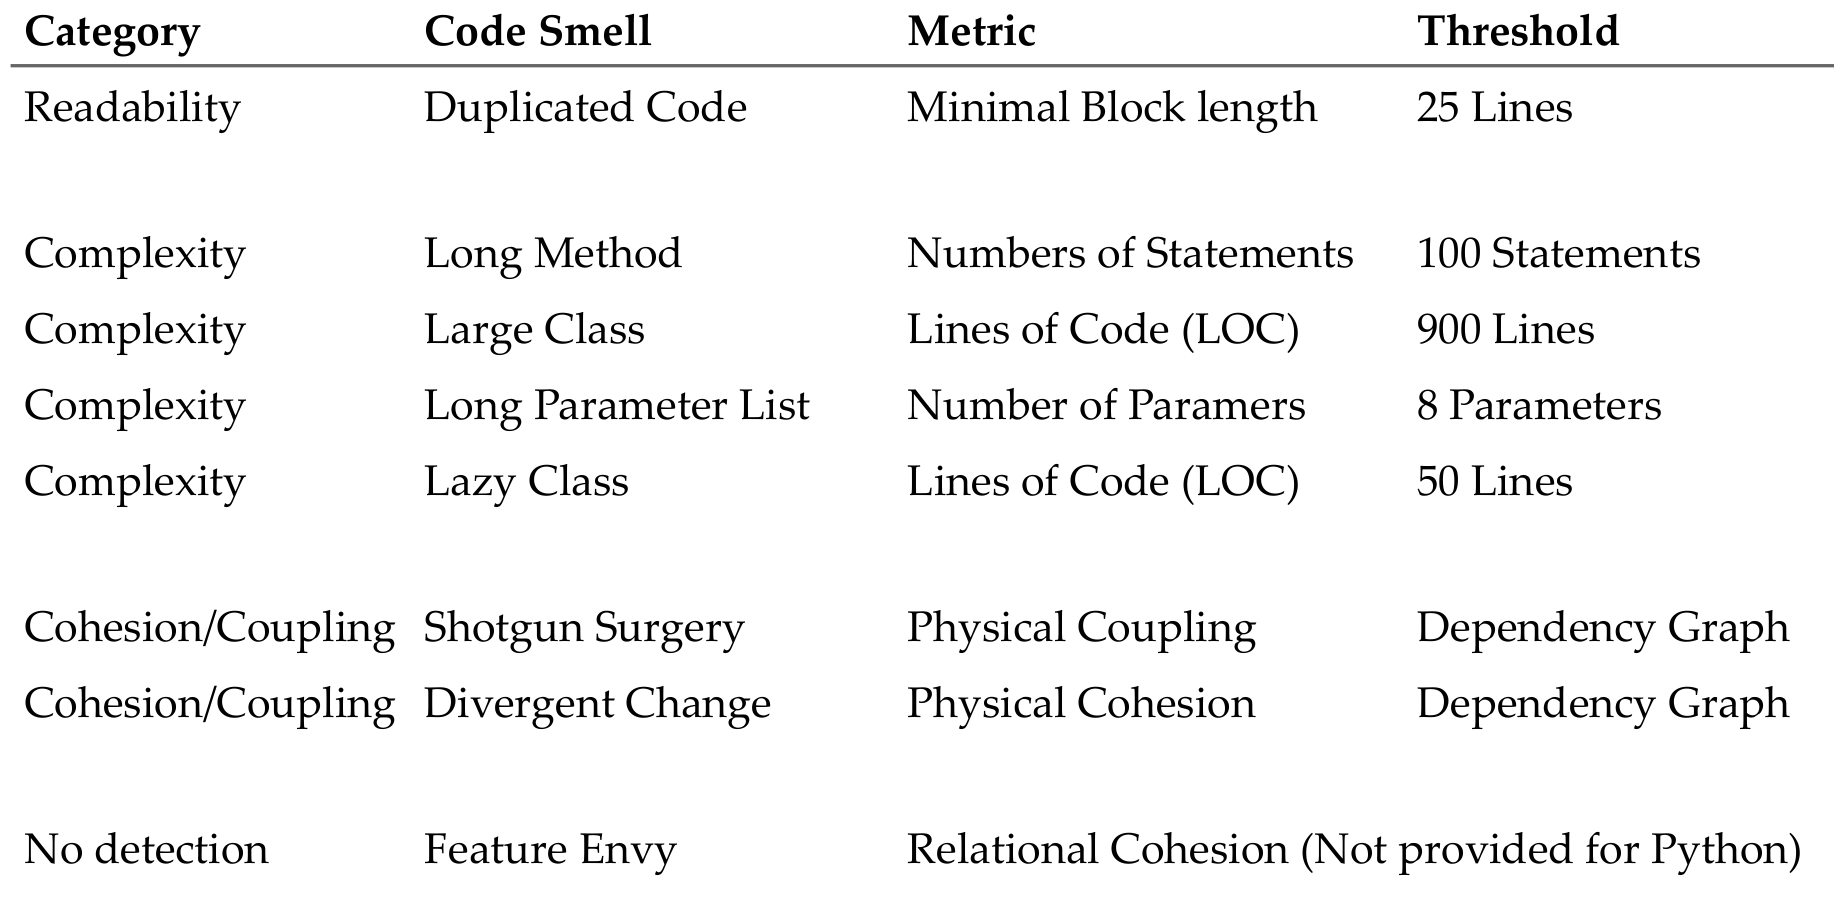
\includegraphics[width=\textwidth]{./assets/smell_overview}
    \caption{Metrics without prioritization}
\end{figure}
% Table
The above table presents for each code smell a corresponding metric. In addition, for some metrics, a threshold value is given. When the threshold value is surpassed, there is an indication that this code smell exists in the software system.

% Subgroups
Individual metrics are categorized into three subgroups, named after the quality attribute they best represent. More importantly, however, this distinction is made, as each of the group differs in regard to how a metric results in a smell detected. 

% Duplicated Code -> Automated
Duplicate code particularly differs from the other smells, due to it being detected automatically. Previously, it was stated that it was difficult to find appropriate tools to detect code smells, due to lack of availability.
In the case of code duplication, this is however readily available because detecting code duplication can be done language agnostic. In order to detect duplication of code in programs, the software does not need to understand the programming language. For instance, this same mechanism could be applied to other types of text that are not code.

% Complexity -> Threshold
Half of the code smells, in the subgroup called complexity, follow a typical metrics based approach. The threshold value indicate when a code smell is potentially present. Notably, all the metrics in this category involve counting of some sorts. In particular, the smells are detected by counting the number of statements, lines of codes, and numbers of parameters of methods. Prioritization of given smells can be done by comparing the extent of how much a given threshold value is surpassed. Similarly, code smells can be discarded if the associated metric does not surpass the threshold value. 


% Cohesion/Coupling -> Dependency graph
Lastly, Shotgun Surgery and Divergent change respectively are bound to the coupling and cohesion of the software system. Here the incoming / outcoming [...] is measured. The metric physical coupling ...
[describe the difference]
The appropriate threshold value highly depends on the size of the software system. The larger the code base, generally more ... will be expected. Therefore, the author decided to use a dependency graph in order to make the decision of whether these two smell are prominent throughout the codebase. 


\section{Testing}
% Transition
In the section that follows, it will be argued that testing is a fundamental part of the refactoring process. In the context of the thesis, it moves on to describe in greater detail the challenges that occur when testing a cyber physical system. In the section that follows, the methods used for testing 
will be outlined, which draw together previously discussed challenges.

\myparagraph{Importance of Testing in a Refactoring Process}

% Importance of Tests
Moving on now to consider, in what ways, testing plays an important role in the refactoring process. In order to understand the significance, it is appropriate to return to the subject of Martin Fowler's definition. According to his definition, refactoring does not alter the external behavior of code {fowler2018}. It was pointed out in the theoretical part of this paper that by not changing the features of the program, programmers can alleviate the risks associated with changing the codebase, which mainly includes the creation of new bugs. Because of this, one can immediately understand how testing is required during refactoring. In more concrete terms, if we want to find out whether the behavior of the code base did not alter, we use testing to confirm this notion. 

% False perception
Further, confirming an unaltered state of code behavior is vital to verify the improvement of code quality. Disregarding testing is likely to result in a false perception of code quality, as bugs are not taken in consideration. In other words, testing can ensure that the software system is in a better state than before, given the quality metrics have improved.

% Mistakes
Allen Holub demonstrates these risks with the statement that "Refactoring without tests is like crossing a busy street blindfolded" (Allen Holub). Similarly, Fowler [p.~59]{fowler2018} argues, mistakes naturally occur and are not a problem if caught quickly. Further, in regard to refactoring he mentions the significance of self-testing code, which allows making it much safer to add new features without breaking anything.

\myparagraph{Testing Cyber Physical Systems}



% CPS Challenges
Having defined the importance, it is now necessary to explain the present challenges given that our software system being a cyber-physical system (CPS). The different characteristics of CPS also needs to be taken into account when determining the methodology of testing these systems. Robots and other cyber-physical systems react to information from the physical worlds and must operate safely even in the presence of uncertainties {geissvolkermaria}. In such a dynamic real-world environment, Kapur {kapurpulkit2020} describes testing, whether a robot will behave as expected, as a time-consuming and complicated task for developers. {raikumar2010} points out the challenge of the heterogeneous nature of CPS, making it difficult to verify and validate the software systems. Similarly, {abbaspourasadollah2015} mentions that defining the boundaries and physical limitations of the test landscape is a challenge in testing a CPS. Another limitation in CPS testing is using an automated semi-automated method. Here, the efficacy of testing is limited by the element of its hardware components. Testing is then dependent on hardware operating appropriately and therefore including the prominence of physical motions subject to considerable time necessary for each test run. The lack of available software that mitigate these challenges poses a substantial limitation on the testing within our context. Some challenges, for instance could be mitigated by using a physics-based simulation that mimics the real-world environment. Simulations do exist in practice, but are unavailable for the present software system. 


% Software test -> Manual test
In general, there is a high interest to use automated testing, as manual testing is more likely to produce errors {turlea2019}.  The levels of CPS software testing contains verifying software, hardware, network, and the integration of all these components to work as a single system {abbaspourasadollah2015}. Despite the advantages of automated test, the fact needs to be considered that for the software system at hand, none of these software tests are available. As a result, developing a testing suite for the software system scratch would certainly be out of the scope of this thesis. 

% One advantage
In fact, there exists an advantage of manual testing that is particular to CPS. Indeed, the physical nature of CPS allows the manual testing through visual observation. Moreover, this benefit is especially apparent when taking into account that our software project is focussing on managing entire processes. In other words, we have the ability to detect for any change in behavior by testing a specific process. 

% Justification
Both the lack of software tests and the ability to visually observe behavior changes were the primary motivations that manual testing was chosen as the preferred method. It is still less reliable compared to software testing, but adequate to reach the aims of the thesis. This is due to the fact that, while not guaranteeing the equality of the entire software system, this method can decently predict the equivalence of the software needed for specific processes used for testing. One key factor in this approach is the selection of one or multiple processes that best cover most of the software system. Consequently, the interactions among the individual components can be examine, delivering benefits similar to integration testing. All in all, this approach does not provide the same degree of assurance as comprehensive unit and integration testing. Nevertheless, it is an approach that suits the preconditions within our context. Specifically, we can to a certain degree assume that we did not alter the external behavior within the scope of specific processes. 

\myparagraph{Method selection}

% Transition
As indicated previously, testing for this thesis will be done manually by means of observing an entire process of the CPS. Methods are selected that strive to be able to test objectively and in a routinized manner. Camunda Modeler is used to automate the business processes and the Gherkin Language is used to formulate requirements. Using Camunda Modeler provides objectivity by having a standardized way to run processes. Similarly, the Gherkin language offers a way to objectively formulate requirements. In combination, these tools deliver a procedure to reduce ambiguity, which is essential in order to capture any cues in observable changes. Having this standardized approach allows us to alleviate some shortcoming of manual testing, while also reducing human error.

% What we have
=== Visualization: Camunda Screenshot ===

Even though there are no software tests available, multiple business processes in using the BPMN representation have already been implemented for the present software system. These representations stored in files are what is being executed by the Camunda Modeler and allow the automation of the processes.  In particular, we use a process stored in the file \emph{production\_process.bpmn}. Using this file, we are able to simulate an entire production process that includes all components of the factory and hence the can cover a major part of the software system. Using the contents of this file, the Camunda Modeler is able to sequentially do the specified HTTP requests that would otherwise have been done manually. Performing these requests manually would not only be very tedious, but also introduce ambiguity. In addition, the BPMN notation used by Camunda Modeler allows us to visually inspect at which part of the process one currently is when running it. This is a fundamental feature, when trying to find out where a current issue might be located.


% Gherkin Explanation
Gherkin on the other hand is not a software solution. Instead, it is a language that is oftentimes used in conjunction with other software tools. Hereby, one can formulate behavior in the form of specifications written in plain text and understandable by humans. It uses a set of special keywords that enables formulating these specifications in a structured way (https://cucumber.io/docs/gherkin/reference/). We can then validate whether the software does what the specifications say. The validation is oftentimes done with writing related software tools. However, in our context this will be done manually. Consequently, using the gherkin language, we are able to objectively check whether the current codebase still fulfills the specification in a form that is human-readable and can also be routinely repeated in a standardized way. 

=== Visualization: Gherkin as code syntax ===

Language
- Feature: 
	High-level description of Application
- Scenario Steps: 
	Action to be performed by a user
	Expected Results of the action
- Scenario Syntax
	Given (preconditions)
	When (user action)
	Then outcome)
	And (multiple statements)

As seen in the specifications above, one can observe multiple prerequisites that are necessary due to having hardware. This amount of detail is critical when wanting to reproduce this process at a later time. Even though, some specifications might seem self-evident, only then we can diminish the ambiguity associated with testing CPS. 

% Optional: DEBUGGING
% - Previous stated tool is what we use to periodically check AFTER we did refactoring
% - There are preventative measure one can take DURING the refactoring. For instance bugs can be caught by trying to run python code, and see whether errors are raised
% - At current time, a lot of issues can be caught during programming itself with modern IDEs
% - With an IDE (Integrated Development Environment) Formatters and static type checkers are also able to catch bugs in the code writing process. 
% - During programming I use the pyright server as a static type checker
% - In order to early detect errors before program execution
% - Advantage is that we do not need to tediously run code all the time, but can catch them before running.
% - Don't need to run code to see malfunctions within the code
% - No errors obviously do not mean that there are no bugs. There could still be unexpected behavior.
% 	-> This is especially the case with python (statically typed language, polymorphism) == Means debugging alone would not suffice, testing is key



\section{Measuring Improvement}
[Need to remove readability]

% Transition
Having incorporated testing in our refactoring model, we are now in a position to consider methods for measuring the improvement of its quality. As mentioned in the theoretical framework, to measure the internal quality, programmers can consider quality attributes as measurement criteria. Here the assumption is that with proper correct refactoring these quality attributes are improved.

\myparagraph{Importance}

% Importance of tracking
Measuring improvement in code quality, allows us to evaluate how successful a refactor was. By means of comparing the refactored software system with its state prior to the refactoring, we are able measure this effect. Having such measurements aids us in making decisions in the future. If the metrics are sufficiently accurate, one could simply argue when to initiate and when to stop refactoring, on the sole basis of these measurements. The comparison of the initial and final state of a refactoring can be further extended by periodically measuring code quality. It is clearly useful to know, by refactoring which code smell, affected code quality the most. Through continuous measurements we are able to answer this question. We then have a basis to argue the amount of which refactoring contributed to the improvement of quality. 

% Two indeces
In order to quantifiably measure the improvements, the thesis will focus on two metrics. First and foremost, it will make use of the maintainability index, which measures how maintainable the source code is. Another focus of the measurement is to analyze the readability of the code. Here, a rating index is provided by a quality checker called pylint. It computes a rating between with a maximum of 10 that is focussed on the PEP 8 python standard. These two indeces have been chosen primarily, as they both provide a single-valued quantification of code quality. In addition, the combination of the two allows us to first evaluate the codebase from a more wide perspective by means of looking at the maintainabilty index and second from a more narrow perspective in terms of its readability. A more detailed account of the indeces will be given in the following section.

\myparagraph{Maintainability Index}

% Introduction
For the computation of the maintainability index the python package Radon is used. Apart from the maintainability index, this software tool is able to compute raw metrics (SLOC, comment lines, blank lines), cyclomatic complexity and halstead volume. These are not random metrics, as the maintainability index does actually include all of these in its computation. The documentation of Radon provides brief explanations of the index and its components. The following section makes extensive use of the documentation in order to provide an overview.

[Include Radon Documentation]


Original Formula:
\begin{equation}
\mathrm{MI}=171-5.2 \ln \mathrm{V}-0.23 \mathrm{G}-16.2 \ln \mathrm{L}
\end{equation}

\begin{itemize}
\item V = Halstead Volume
\item G = Cyclomatic Complexity
\item L = Source Lines of Code (SLOC)
\end{itemize}

Derivative (used by Radon):

\begin{equation}
\mathrm{MI}=\max \left[0,100 \frac{171-5.2 \ln \mathrm{V}-0.23 \mathrm{G}-16.2 \ln \mathrm{L}+50 \sin (\sqrt{2.4 \mathrm{C}}))}{171}\right]
\end{equation

Both formulas calculate the maintainability as a factored formula consisting of three primary components. Halstead volume is measured by multiplying halstead length (number of operators and operands) with vocabulary (number of unique operators + unique operands) Cyclomatic Complexity calculates a the number of linearly independent paths in the source code, indicating the complexity of a program. SLOC counts the number of lines in the computer program.

The original equation is included to easier understand what the formula wants to achieve. The second formula, which is used by Radon, is a derivative of the original formula. However, the second formula is preffered as it is able to measures the maintainability between a scale from 0 to 100. Consequently, the computation is easier to understand, as higher values indicate better maintainability. The second difference is that this formula also takes into account the percentage of commented lines indicated by the variable \emph{C}. It presumably is included to offset SLOC, when the source code contains a lot of commented lines.

\myparagraph{Methods used for taking measurements}

The method of taking measurements is also a design decision that was consciously carried out. At first, taking the measurements manually was considered suitable enough. Still after some consideration it was clear that an automated approach deemed much more appropriate. Reasons for this choice includes that manually running the software tool after each change quickly becomes tedious. It would be considerably time inefficient and can at the same time be quickly forgotten. There would be no clear indication on the right amount of measurments to take in a routinized way. If too many measurements are taken it requires a lot of time and it is difficult to differentiate between the individual measurements. Conversl, if too few measurements are taken, there would be no sufficient information available to make meaningful conclusions.

After careful reflection, it become evident that a suitable way of taking measurements would be to take them after each commit to the version control tool git. That way each measurement could directly be attributed to every commit, which includes the necessary information on code changes. Luckily there is a way to write so called hooks, that enable to run a script in conjunction with git activities. Consequently, a git hook, written as a bash script, could be implemented that is executed prior to each git commit. This way both concerns of time inefficiency and lack of attribution could be ressolved. It is important to not however, that this is only possible due to Radon being a command line utility. If graphical software would have been used, only a manual approach would have been possible, if not implemented by the software itself.

The bash script performs to functions. Initially it executes radon to compute the maintainability index and its subcomponents. Here, the result is temporarily saved in a variable. Next, these computations are written to a file, which is saved locally on the computer. The files are named with the date and time of execution which allows the indicated attribution between measurement and commit. The design of this methodology enables continuous tracking in three dimensions. First, we are able to attribute individual refactoring steps in the form of commits. Second, we are able to more broadly connect measurements to the refactoring of individual code smells. This allows us to measure how getting rid of each smell improved the overall maintenance index. Lastly, by comparing measurements to the initial state of the project, we can evaluate what the overall progress regarding the entire project is up to a certain point in time.

% % CONCLUSION

% % Reasons for chosing it
% - According to the issues, the methodological part of this part should in practice be more extended in order to achieve more meaningful measurements.
% - Maintainability Index is Able to measured on a file-per-file basis.
% - Because it is one index that includes a variety of indeces (to better estimate the overall maintainability)
% - Misconsception that the more advanced the programmer, the more complex the code will be. However, advanced programmers should strive to produce the simplest, elegant and easy to read programs that will achieve the objective with the least amount of steps.
% - New features request are keep coming and we are adding new code to the code base. The code base grows exponentially. 
% - The author  do  not  claim  that  the  the  MI  is  the  only  model  for  predicting  maintainability,  nordo  we  claim  it  is  the  best  overall.  
% - Chosen because of on the one hand is simple (One Value), and on the other hand measures a lot of things
% 	-> Measuring more broadly allows not to fall into the trap of self fulfilling prophecy
% 	-> This trap is apparent in the readability rating (but we are aware of it)

% % Reasons for extending to more metrics
% - It is very good that with one metric we are able to have a lot of characteristics that fit very well for the thesis
% - There are however a lot of of downsides for this especial metric, which resulted in some criticism of this metric
% - The maintainability metric should not be taken into account as seriously as a more comprehensive selection that takes into acocunt the conditions for a specific software system

% - List Shortcoming from articles
% 	-> Some of the shortcomings to be noted include
% 		-> Lack of explanation on the weights

% - The point of this study is not to optimize the metrics but to improve the internal state, these metrics are ultimately just a means of reflection / accountability.
% - Metric does not directly measure the code smells (only in part)
% - The above described methods apply much better if a whole team is refactoring a multitude of smells over a longer period of time

% Justification
% - In addition, one of the most important metrics is getting rid of code smells. The amount of code smells reduced, will mean the amount of internal problems solved.
% - This methodAccording to the issues, the methodological part of this part should in practice be more extended in order to achieve more meaningful measurements.

% How the measurements are taken is also a design decision that was taken (bewusst). First, taking the measurements manually after some time deemed approprate. After some consideration however an automated approach was deemed more appropriate. Reasons for this choice included ... however does allow us to not rely on getting rid of code smells alone as a measurement of success, but using the quality attributes.
% - An example for this false perceived notion, eliminating a large class, that however makes the code more difficult to understand, is a downgrade

% - From the individual parts of the refactoring process, this part would need the most work. Due to the fact that it doesn't directly infuence the quality of the refactoring its not that big of a problem.
% - It however as argued in the beginning of the chapter can not be left out / ignored and is thus despite its shortcomings still included. Can serve as an illustration.
% - Therefore, all in all, these methods of measurement show to be promising and especially meet our demands very well.


\section{Refactoring}

\myparagraph{Methods used for Refactoring}

[Write this after doing the refactoring]

- This rather simple set of tools does not include the details of the implementation of refactoring 
- A more detailed account on this topic is given in the next chapter, where individual refactoring steps are documented

\myparagraph{Limitations}

- Recap this chapter with a conclusion
- How this detailed preparation of refactoring is important, compared to when just entering it
- In practice not this comprehensive, but most is developed over time as an intuition through experience
- It is however advantageous to formulate it down, making us able to discuss the topic and develop an optimal strategy
